\subsection{Overview}
	Computer simulation is getting popular in the field of science. Individuals tackle diverse experimental issues using computer control through simulating artificial testing environments. They use these simulated environments to test scientific models in order to prove or disprove their feasibility and correctness.
	 
	Today's high machine power gives people the capacity to simulate environments at a rate much quicker than any real environment, thus any experiment carried out in the simulated medium would provide results minutes, hours, days and often weeks, months and years ahead of what the same experiment would provide if executed in the real world.
	
	One of the frameworks or systems that are best considered using a computer simulation is a traffic network. It is typical to experiment with traffic networks in a computer-simulated environment because experimenting with traffic in the real environment is impractical. 

\subsection{Simulation models}
	A typical classification method for simulation models is based on the variability content that represents the deterministic nature of simulation that represents the static or dynamic characteristics of simulation. Regarding how frequent the activity of the traffic network is updated and the statistics on traffic performance is collected, the most frequently used classification method is based on the details a model intends to simulate, namely, microscopic or macroscopic modelling.
\subsubsection{Microscopic modelling}
	Microscopic simulation modeling methods are based on car-following and lane-changing theories, which can represent the traffic operations and vehicle/driver behaviors in detail. The car-following theory describes the longitudinal movement of vehicles. The classical car-following approach is quite straightforward, i.e., each vehicle attempts to advance at its desired speed while maintaining a safe following distance from the vehicle ahead. [4] Microscopic simulation modelling incorporates queuing analysis, shock-wave analysis, and other analytical techniques.
\subsubsection{Macroscopic modelling}
	Macroscopic models do not consider car-following behaviour in detail, but instead model traffic as an aggregate fluid flow. To better understand the collective behaviour of traffic and analyse flow conditions in a dynamic fashion, continuum models, either simple or high-order, are usually employed in macroscopic simulation modelling. The simple continuum model consists of a continuity equation representing the relationship between the speed, density, and flow generation rate. [5] Although the existing high-order models look promising, they have not as yet proved truly superior to the simple continuum models at least in medium-to-congested flow conditions [6]
\subsection{Comparison of different traffic simulation packages}
	We will briefly review the following well known and widely used simulation packages;
	
	\begin{itemize}
		\item Simulation of Urban Mobility (SUMO)
		\item Quadstone Paramics Modeller
		\item Aimsun
	\end{itemize}

\subsubsection{Simulation of Urban Mobility (SUMO)}
	Simulation of Urban Mobility (SUMO) is an open source, very compact, microscopic road traffic simulation package designed to handle large road networks. [1]
	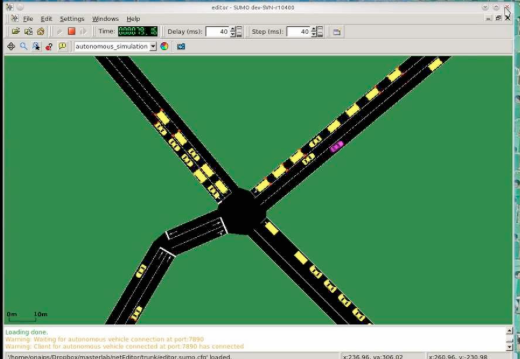
\includegraphics[scale=0.7]{./images/SUMO.png}
	The simulation platform SUMO's features include:
	\begin{itemize}
		\item Microscopic simulation – vehicles and public transport are modelled explicitly.
		\item Simulation of multi-modal traffic, e.g., vehicles, public transport and pedestrians.
	\end{itemize}
